% fundDiff.tex      pdflatex ZhCvGo15
% Diffuse globally, compute locally: a cyclist tale
% Tingnan Zhang, Daniel I. Goldman and Predrag Cvitanovi\'c

%\subsection{Fundamental domain diffusion tensor}
%\label{s-fundDiff}

If a quantum system has an underlying symmetry, its Hamiltonian can be
block-diagonalized by the irreducible representations of the symmetry
group, with each block spanned by a set of degenerate states. In fact,
this standard approach is not specific to quantum mechanics. Once we
describe the classical dynamics in terms of the \evOper, the algebra
follows in a similar way, and the group factorization applies. The
quotiented {\statesp}, \ie, the fundamental domain, is more compact,
as understood by the one-to-many map of \po s. The
convergence of cycle expansion formulae improves and less cycles are
required.  In previous works~\rf{CGS92,DasBuch} fundamental domain
cycle expansion results for scalar quantities such like Lyapunov
constant have
been
obtained. However, for reasons mentioned in
\refsect{s-FundTranslation}, an exact formula for the diffusion
constant (an average over displacement, a vector quantity) was
not given.


We start from the trace of elementary cell \evOper\
\refeq{eq-trace-disc} and project it into the irreducible
representations $\II_G$. We first derive the map version:
\bea
\tr{\cal L}^n &=& \sum_{\alpha \in\II_G} \tr{\cal
L}_{\alpha}^n\nonumber\\ \tr{\cal L}_{\alpha}^{n} &=&
\frac{d_\alpha}{|G|}\sum_{h \in
G}\chi_\alpha(h)\nonumber\\&&\int_{\t {\cal M}} d\tx
\sum_{\sigma \in G}\delta (h^{-1}\tx -
f^n(\sigma\tx))e^{\beta\cdot\left(\hat{f}^n(\sigma\tx)-\sigma\tx\right)}
\,,\nonumber
\label{eq-trace-ir}
\eea
where $d_\alpha$ is the dimension of irrep $\alpha$ and
$\chi_\alpha(h)$ the group character. Using equivariance relations
\refeq{eq-equivariance-flow}, \refeq{eq-equivariance-disp}, and
noting that the little group is closed, we have:
\bea
\tr{\cal L}_{\alpha}^{n} &=& \frac{d_\alpha}{|G|}\sum_{\sigma \in
  G}\sum_{h \in G}\chi_\alpha(h)
  \nonumber\\
  &&\int_{\t {\cal M}} d\tx \delta (h^{-1}\tx -
f^n(\tx))e^{\beta\cdot\sigma\cdot(\hat{f}^n(\tx)-\tx)}\,.
\label{eq-trace-ir-disc}
\eea

As in the analysis of \refsect{s-POT}, the $\delta$-function part
$\delta (h^{-1}\tx - f^n(\tx))$ in the integral  selects points on
fundamental domain relative \po s $\tp$. In addition, after
completing the cycle $r$ times, the cumulative group action should
also satisfy $h^{r}_{\tp}(\tx) = h$. It follows that the integral in
\refeq{eq-trace-ir-disc} can be written as a sum over fundamental domain
cycles
\beq
\int_{\t {\cal M}} = \sum_{\tp}\delta_{n, n_pr}\sum_{\tx\in
\tp}\delta_{h^r_{\tp}(\tx), h}
\frac{e^{\beta\cdot\sigma\cdot\hat{L}_\tp(r,
\tx)}}{\vert\det\left({\bf 1 - J}_\tp^r(\tx)\right)\vert}\,,
\label{eq-trace-ir-expan}
\eeq
where the $r-$repeats displacement $\hat{L}_\tp(r, \tx)$ along the
orbit takes the form computed in~\refeq{eq-fd-displacement},
and ${\bf J}_\tp^r(\tx)$ absorbs the cycle group element
$h^r_{\tp}(\tx)$. The spectral determinant for the $\alpha-$irrep is:
 \beq
Z_{\alpha}(\beta,z)
=\exp\left(-\frac{d_\alpha}{|G|}\sum_{\sigma\in
G}\sum_{\tp}
\frac{1}{\cl{\tp}}\sum_{\tx\in\tp}\sum_{r=1}^{\infty}
t_\tp(r, \tx)
\right)\,,
\label{eq-fd-zeta}
\eeq
where
\beq
t_{\tp} =\frac{z^{n_\tp r}{\chi_{\alpha}(\hp^{r}(\tx))
e^{\beta\cdot\sigma\cdot\hat{L}_{\tp}(r,\tx)}}}
{r\vert\det\left({\bf 1 - J}_\tp^r(\tx)\right)\vert }
\,,
\eeq
is the weight associated with the orbit.  The corresponding zeta
function $\zeta_\alpha$ is obtained by replacing $\det\left({\bf 1 -
J}_\tp^r(\tx)\right)$ with expanding eigenvalues $\ExpaEig_\tp$.
Eq.~\refeq{eq-fd-zeta} takes a more complicated form than its
counterpart~\refeq{eq-det-cont} in the elementary cell. As a sanity
check, note that if the little group contains only the identity
element $e$, i.e. there is no additional symmetry, it is reduced to
\refeq{eq-det-disc}. Generalization to continuous flow is also
different. Besides replacing $z^{n_p}\to e^{-s\period{\tp}}$, the
summation is changed to an integral
\beq
\frac{1}{n_{\tp}}\sum_{\tx\in\tp}\to
\frac{1}{\period{\tp}}\oint_{\cal P}d\tau\tx(\tau)\,,
\label{eq-orbitsum}
\eeq
which runs along the tangent (marginal) direction of the orbit. Here
comes an interesting discovery (to which we return in
\refsect{s-numerics}): changing the sum to the integral will produce
\emph{different} results for any non-trivial symmetry (the group of
which contains more than $e$). For consistency, we denote
$\langle\rangle_{\tp}$ as the average over the cycle $\tp$.

The important long term dynamics is contained in the one-dimensional,
symmetric representation: $d_\alpha = 1$ and all $\chi(h)=1$. The
cycle averaged mean drift vanishes,
\bea
\langle\hx\rangle_{\cal \zeta_\alpha} &=& -\left.\frac{\partial
Z_\alpha}{\partial
\beta} \right\vert_{\beta = 0, s = 0} \\\nonumber
&=& Z_\alpha (0, 0)\sum_{\tp}\sum_{r=1}^{\infty}\frac{1}{\vert
G\vert}\sum_{\sigma\in
G} \frac{\left\langle\sigma\cdot
\hat{L}_{\tp}(r,
\tx)\right\rangle_{\tp}}{r\vert\ExpaEig_\tp\vert^r}\equiv
0\,,
\eea
because directions of $\sigma\cdot \hat{L}_{\tp}(r, \tx)$ cancel
each other when we sum the group elements $\sigma$. Observing
that the length  $\vert \sigma\cdot \hat{L}_{\tp}(r, \tx) \vert$ does
not change under isometric transformations, the cycle averaged mean
squared displacement (MSD) is:
\beq
\langle\hx^2\rangle_{\cal \zeta_\alpha} = \prod_{\tp}\left(1 -
\frac{1}{\vert\Lambda_\tp\vert}\right)
\sum_{\tp}\sum_{r=1}^{\infty} \frac{\left\langle\vert\hat{L}_{\tp}(r,
\tx)\vert^2\right\rangle_{\tp}}{r\vert\ExpaEig_\tp\vert^r}
\,.
\label{eq-fd-msd}
\eeq
The formula contains infinite series with exponential tail. In numerical
computations we keep the auxillary variable $z$ in
~\refeq{eq-fd-zeta}, expand ~\refeq{eq-fd-msd} as a polynomial and
then truncate it according to the topological length of the longest
periodic orbit found~\rf{DasBuch}.

\begin{figure}
	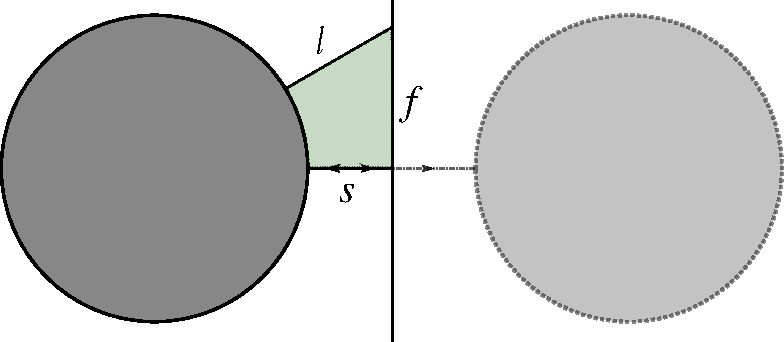
\includegraphics[width=0.45\textwidth]{diffuseTwoDiskBouncing}
	\caption{Fundamental domain fixed point $\{{\bar{0},
			\underline{5}}\}$. The cycle remains entirely on the
			symmetry line $s$, and pivots about $f$.}
	\label{fig-twodisk}
\end{figure}

There is one further technical detail to take care of before we can apply
\refeq{eq-fd-msd} to numerical evaluation of the diffusion constants of the
Lorentz gas system.
In general, one also has ``boundary cycles,'' \ie, \po s which are completely
contained within invariant subspaces, such as the Lorentz gas lattice symmetry
lines. An example of such cycle is $\cycle{06}$ in elementary cell (or
$\{{\bar{0},\underline{5}}\}$, in fundamental domain symbols),
~\reffig{fig-twodisk}.
Boundary cycles remain unchanged when we apply
the group action that reflects about the symmetry line, thus
simultaneously contribute to multiple terms in
\refeq{eq-trace-ir-expan} (remember that the group element is included
into the Jacobian). Because under axial reflection the eigenvalues
do not flip signs
    \PC{2019-01-20} {
    Not sure about this, removed for now:
(see the Jacobian matrix for in chapter 9 of~\refref{DasBuch}),
    }
in our system the boundary orbits contribute
do not require a special treatment
(see ChaosBook Chapter~{\em Discrete symmetry factorization}\rf{CBsymm}).
% chapter 25 of ~\refref{DasBuch}).
